%\documentclass[xcolor=dvipsnames]{beamer}
\documentclass[xcolor=dvipsnames,handout]{beamer}

\setbeamertemplate{blocks}[rounded][shadow=true]
\usepackage{etex}
\usepackage{xcolor}
\usepackage{colortbl}
\usepackage{multirow}
\usepackage{amsmath}
\usepackage{amsfonts}
\usepackage{epsfig}
\usepackage[english]{babel}
\usepackage{colortbl}
\usepackage{multirow}
\usepackage{fancyvrb}
\usepackage{bm}
\usepackage{hyperref}
\usepackage{caption}
%\usepackage{subcaption}
\usepackage{graphicx}
\usepackage{multicol}
\usepackage{epsdice}

\definecolor{newred}{RGB}{127,0,0}
\let\iitemize=\itemize \let\endiitemize=\enditemize \renewenvironment{itemize}{\iitemize \vspace{1mm} \itemsep2mm}{\endiitemize}
\let\eenumerate=\enumerate \let\endeenumerate=\endenumerate \renewenvironment{enumerate}{\eenumerate \vspace{1mm} \itemsep2mm}{\endeenumerate}
% == theme & colors
\mode<presentation>
{


\usetheme[progressbar=frametitle]{metropolis}
\usecolortheme{beaver}
  \setbeamercovered{invisible} %or transparent
  \metroset{block=fill}
  \setbeamercolor{block title example}{fg=gray!40!black}
  \setbeamercolor{itemize item}{fg=gray!40!black} 
  \setbeamercolor{title}{fg=newred} 
}

      
\setbeamercolor{background canvas}{bg=white}


\usepackage{tikz}
\usetikzlibrary{shapes,decorations,arrows,calc,arrows.meta,fit,positioning}
\tikzset{
    -Latex,auto,node distance =1 cm and 1 cm,semithick,
    state/.style ={ellipse, draw, minimum width = 0.7 cm},
    point/.style = {circle, draw, inner sep=0.04cm,fill,node contents={}},
    bidirected/.style={Latex-Latex},
    el/.style = {inner sep=2pt, align=left}
}
    

% === if you want more than one slides on one page ===
\usepackage{pgfpages}



\title{Mathematics for Data Science}
\subtitle[]{Lecture 12: Linear Regression and Wrap-Up} 
\author[Asya Magazinnik]{Asya Magazinnik}
\institute{Hertie School}
\date{\today}

\renewcommand\r{\right}
\renewcommand\l{\left}
% \newcommand\sign{{\rm sign}}

%% == change spacing for itemize
%\let\oldframe\frame
%\renewcommand{\frame}[1][1]{
%\oldframe[#1]
%\let\olditemize\itemize
%\renewcommand\itemize{\olditemize\addtolength{\itemsep}{.25\baselineskip}}
%}



\def\insertnavigation#1{\relax}
% \usefonttheme{serif}
\usepackage[all]{xy}
\usepackage{geometry,colortbl,wrapfig}
\usepackage{tikz}  
\usepackage{graphicx,setspace,subfigure}
\usepackage{epstopdf}
\DeclareGraphicsRule{.tif}{png}{.png}{`convert #1 `dirname #1`/`basename #1 .tif`.png}
\newcommand{\Ex}{\textsc{Example  }}
\newcommand{\series}{\sum_{n=1}^{\infty}} 
\newcommand{\ball}[1]{B( #1)} 
\newcommand{\inner}[1]{\ensuremath{\langle #1 \rangle}}
\newcommand{\e}{\epsilon}
\newcommand{\grad}{\nabla}
\newcommand{\pa}{\pause \item}
\newcommand{\bi}{\begin{itemize}}
\newcommand{\ei}{\end{itemize}}
\newcommand{\be}{\begin{enumerate}}
\newcommand{\ee}{\end{enumerate}}
\newcommand{\R}{\mathbb{R}}
\newtheorem{proposition}{Proposition}
\newtheorem{axiom}{Axiom}
\newtheorem{assumption}{Assumption}
\newtheorem{remark}{Remark}
\newcommand{\matr}[1]{\bm{#1}}     % ISO complying version



\newcommand{\indep}{{\bot\negthickspace\negthickspace\bot}}

\begin{document}

\subject{Talks}
\AtBeginSection[]
{
  \begin{frame}[plain]
    \frametitle{}
    \tableofcontents[currentsection]
    \addtocounter{framenumber}{-1}
  \end{frame}
}

\AtBeginSubsection[]
{
  \begin{frame}[plain]
    \frametitle{}
    \tableofcontents[currentsection,currentsubsection]
    \addtocounter{framenumber}{-1}
  \end{frame}
}


\frame[plain]{
  \titlepage
  \addtocounter{framenumber}{-1}
}

\begin{frame}{Why Linear Regression}
    \begin{itemize}
        \item Easy and informative
    \item A useful jumping-off point
    \item Many fancy statistical learning approaches can be seen as generalizations or extensions of linear regression
    \end{itemize}
\end{frame}

\begin{frame}{Linear Regression Can Tell You A Lot}
\vspace{2mm}
Imagine you're a statistical consultant hired to advise a company on their marketing strategy. They might wish to know: 
\begin{enumerate} 
\small 
    \item Is there a relationship between advertising budget and sales?
    \item How strong is the relationship between advertising budget and sales? 
    \item Which media are associated with sales? (e.g. TV, radio, newspaper)
    \item How large is the association between each medium and sales? 
    \item How accurately can we predict future sales? 
    \item Is the relationship between advertising and sales linear? 
    \item Is there synergy among the advertising media? 
\end{enumerate}
\end{frame}

\begin{frame}{Linear Regression Setup}
\[ 
\text{sales} \approx \beta_0 + \beta_1 \times \text{TV}
\]
\pause 
\[
\hat{\text{sales}} = \hat{\beta}_0 + \hat{\beta}_1 \times \text{TV}
\]
\pause
\[
\text{sales} = \hat{\beta}_0 + \hat{\beta}_1 \times \text{TV} + e
\]
\pause 
\[
\text{sales} = \hat{\text{sales}} + e 
\]
\end{frame}

\begin{frame}{Linear Regression Setup}
\vspace{5mm}
    \centering    \includegraphics[width=\textwidth]{images/sales.png}
\end{frame}

\begin{frame}{Linear Regression Setup}
The linear regression optimization problem is to \alert{minimize the residual sum of squares}:
\begin{align*}
    \text{RSS} &= \sum_{i=1}^n e_i^2 \\
    &= e_1^2 + e_2^2 + ... + e_n^2 \\
    &= (\text{sales}_1 - \hat{\beta}_0 - \hat{\beta}_1 \text{TV}_1)^2 \\
    &+~   (\text{sales}_2 - \hat{\beta}_0 - \hat{\beta}_1 \text{TV}_2)^2 \\
    &+ ... \\
    &+~   (\text{sales}_n - \hat{\beta}_0 - \hat{\beta}_1 \text{TV}_n)^2 
\end{align*}
\end{frame}

\begin{frame}{Set Up the Minimization Problem and Solve}
    \[ \min_{\hat{\beta}_0, \hat{\beta}_1} \sum_{i=1}^n e_i^2 = \min_{\hat{\beta}_0, \hat{\beta}_1} \sum_{i=1}^n (y_i - \hat{\beta}_0 - \hat{\beta}_1 x_i)^2 \] 
    \\
    \vspace{60mm}
    \vfill
\end{frame}

\begin{frame}{Solutions to the Problem}
\begin{align*}
    \hat{\beta}_0 &= \bar{y} - \hat{\beta}_1 \bar{x}_i \\
    \hat{\beta}_1 &= \frac{\sum_{i=1}^n (x_i - \bar{x}) (y_i - \bar{y})}{\sum_{i=1}^n (x_i - \bar{x})^2} 
\end{align*}
\end{frame}

\begin{frame}{From One Covariate to Many}
\[
\hat{\text{sales}} = \hat{\beta}_0 + \hat{\beta}_1 \times \text{TV} + \hat{\beta}_2 \times \text{Radio} + \hat{\beta}_3 \times \text{Newspaper}
\]
\includegraphics[width=\textwidth]{images/multiple_reg.png}
\end{frame}

\begin{frame}{}
\centering
\vspace{2mm}
\includegraphics[width=.9\textwidth]{images/two_covar.png}
\end{frame}

\begin{frame}{Is at least one predictor useful in predicting the response?}
    \includegraphics[width=\textwidth]{images/fstat.png}
\end{frame}

\begin{frame}{Further Considerations}
    \begin{itemize}
        \item Variable selection
        \item Model fit
        \item Causal interpretation
    \end{itemize}
\end{frame}

\begin{frame}{Model Fit: Nonlinearities}
    \centering
    \vspace{3mm}
    \includegraphics[width=.85\textwidth]{images/model_fit.png}
\end{frame}

\begin{frame}{Model Fit: Interactions}
    \centering
    \vspace{5mm}
    \includegraphics[width=\textwidth]{images/model_fit2.png}
\end{frame}



\begin{frame}{Causal Interpretation of Regression}
\vspace{2mm}
    \begin{figure}
       \begin{center}
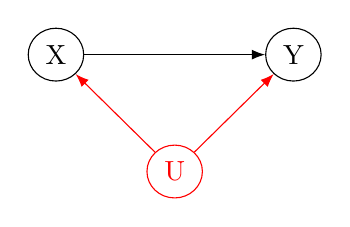
\begin{tikzpicture}
    \node[state] (U) [red] at (0,0) {U};
    \node[state] (X) [above left =of U] {X};
    \node[state] (Y) [above right =of U] {Y};
    \path (U) [red] edge (X);
    \path (U) [red] edge (Y);
    \path (X) edge (Y);
\end{tikzpicture}
\end{center}
\end{figure}
    \begin{itemize} \small 
    \item \textbf{Causal question:} what is the effect of getting a Hertie School degree ($X$) on your earnings ($Y$)? 
        \item \textbf{Confounding:} Your excellent prior academic record ($U$) made you competitive for admission to the Hertie School ($X$), and it also makes you competitive for high-paying jobs ($Y$). 
        \item Naive regression: $Y = \beta_0 + \beta_1 X$
        \item Regression with causal interpretation: $Y = \beta_0 + \beta_1 X + \beta_2 U$
    \end{itemize}
\end{frame}

\section{What's Next?}
\begin{frame}{From Statistical Learning to Machine Learning}
    \alert{Machine learning} generally uses larger datasets and algorithms that can \alert{learn from data} in a more automated, adaptive way.
    \begin{itemize} \small 
        \item You can think of it as statistical learning, where many decisions are taken out of the hands of the analyst
        \item The analyst is in charge of general approaches or algorithms for inference or prediction rather than making the relevant choices directly 
    \end{itemize}
\end{frame}

    \begin{frame}{What's Next for You}
        You now have the skills to go independently learn \alert{any statistical or machine learning technique}, with enough time and patience.
        \begin{itemize}
            \item Try it!
            \begin{itemize}
                \item Logistic regression!  (p. 133)
                \item Linear Discriminant Analysis! (p. 142) 
                \item Support Vector Machines! (p. 367) 
            \end{itemize}
            \item The ISL book and the Bishop book are your friends on this next leg of your journey, along with Kevin Murphy's \textit{Probabilistic Machine Learning} 
        \end{itemize}
    \end{frame}

    \begin{frame}{How to Learn About Statistical Learning}
    \vspace{3mm}
        As things get deeper in complexity, you can't understand every detail of a new method. By necessity, some things will become more black-boxy: 
        \begin{itemize} \small 
            \item Optimization
            \item Computation 
            \item (You will learn more about this in Data Structures \& Algorithms)
        \end{itemize}
        But in general, you will be much more reliant on off-the-shelf methods, i.e. R and Python packages, to do the work for you.
        \begin{itemize} \small 
            \item         But think back to our EM, PCA, and linear regression labs for the intuition, which will always be the same.  
        \end{itemize}
    \end{frame}

    \begin{frame}{How to Learn About Statistical Learning}
      \begin{itemize}
            \item What is the data structure? 
            \item Supervised or unsupervised? 
            \item Prediction or inference?
            \item Parametric or nonparametric? 
            \item Essentially, what is the \textit{shape} of the model being fitted and what is the loss function? 
            \item Bias-variance trade-off? 
            \item What is the optimization technique? 
        \end{itemize}   
    \end{frame}



  \begin{frame}{Parting Wisdom}
\begin{itemize}
    \item From here, you can go farther than you ever imagined.
    \[ \sum_{i=1}^n \text{incremental step}_i = \text{Giant Leap} \]
    \item Be ambitious and creative.
    \begin{itemize}
        \item Your ``field'' is not well defined and that's a good thing. 
    \end{itemize}
    \item You have in your pocket a lens for understanding the world. 
\end{itemize}
    \end{frame}
\end{document}
